%%%%%%%%%%%%%%%%%%%%%%%%%%%%%%%%%%%%%%START PREAMBLE THAT IS THE SAME FOR ALL EXAMPLES
\documentclass{article}

%Required: You must have these
\usepackage{Sweave}
\usepackage{graphicx}
\usepackage{tabularx}
\usepackage{hyperref}
\usepackage{natbib}
\usepackage{pdflscape}
\usepackage{array}
\usepackage{authblk}
\usepackage{gensymb}


%\usepackage[backend=bibtex]{biblatex}
%Strongly recommended
 %put your figures in one place
%\SweaveOpts{prefix.string=figures/, eps=FALSE} 
%you'll want these for pretty captioning
\usepackage[small]{caption}

\setkeys{Gin}{width=0.8\textwidth} %make the figs 50 perc textwidth
\setlength{\captionmargin}{30pt}
\setlength{\abovecaptionskip}{10pt}
\setlength{\belowcaptionskip}{10pt}
% manual for caption http://www.dd.chalmers.se/latex/Docs/PDF/caption.pdf

%Optional: I like to muck with my margins and spacing in ways that LaTeX frowns on
%Here's how to do that
\topmargin -1.5cm    
\oddsidemargin -0.04cm  
\evensidemargin -0.04cm % same as oddsidemargin but for left-hand pages
\textwidth 16.59cm
\textheight 21.94cm 
%\pagestyle{empty}    % Uncomment if don't want page numbers
\parskip 7.2pt      % sets spacing between paragraphs
%\renewcommand{\baselinestretch}{1.5} 	% Uncomment for 1.5 spacing between lines
\parindent 0pt% sets leading space for paragraphs
\usepackage{setspace}
%\doublespacing
\renewcommand{\baselinestretch}{1.8}
\usepackage{lineno}
%Optional: I like fancy headers
%\usepackage{fancyhdr}
%\pagestyle{fancy}
%\fancyhead[LO]{How do climate change experiments actually change climate}
%\fancyhead[RO]{2016}
 
%%%%%%%%%%%%%%%%%%%%%%%%%%%%%%%%%%%%%%END PREAMBLE THAT IS THE SAME FOR ALL EXAMPLES

%Start of the document
\begin{document}

%\SweaveOpts{concordance=FALSE}
\Sconcordance{concordance:sm_doc.tex:sm_doc.Rnw:%
1 223 1}


\bibliographystyle{../../Bibliography/bibstyles/amnat.bst}
\title{Drier soils delay plant phenology across temperate forest and grassland systems} 
\author[1,2,a]{A.K. Ettinger}
\author[3,b]{J.S. Dukes}
\author[4,c]{M.R. Johnston}
\author[5,d]{C.R. Rollinson}
\author[1,4,6,e]{E.M. Wolkovich}

\affil[1]{Arnold Arboretum of Harvard University, Boston, Massachusetts 02131, USA}

\affil[2]{The Nature Conservancy,Seattle, Washington, USA}


\affil[3]{Department of Forestry \& Natural Resources and Department of Biological Sciences, Purdue University, West Lafayette, Indiana 47907, USA}

\affil[4]{Department of Organismic \& Evolutionary Biology, Harvard University, Cambridge, Massachusetts 02138, USA}

\affil[5]{The Morton Arboretum, Lisle, Illinois 60532, USA}

\affil[6]{Forest \& Conservation Sciences, Faculty of Forestry, University of British Columbia, Vancouver, BC, Canada}

\affil[a]{Corresponding author; email: ailene.ettinger@tnc.org; phone: 781-296-4821; mailing address: 73 Wall Street. Seattle, WA 98121, USA }

\date{\today}
\maketitle 
\textbf{Author contributions}: All authors conceived of this manuscript, which began at a Radcliffe Exploratory Seminar in 2016, and all authors contributed to manuscript revisions. AKE and EMW conceived of the idea for the literature review, database compilation, and related Radcliffe Exploratory Seminar, and wrote the manuscript. AKE compiled the datasets; AKE analyzed the data and created the figures.

\textbf{Data Accessibility} 
The data reported in this paper are from the MC3E and ExPhen databases, which are available at KNB \citep{ettinger2018,ettinger2022}

\textbf{Running title} Drier soils delay phenology

\textbf{Key words} global warming, warming experiment, microclimate, phenology, bud-burst, leaf-out, flowering, fruiting, senescence 


\textbf{Paper type} GCB %then New Phytologist or Am Bot

%\textbf{Number of words in abstract} 

%\textbf{Number of words in main text} 

%\textbf{Number of references} 

%\textbf{Number of tables} 0

%\textbf{Number of figures} 


%%%%%%%%%%%%%%%%%%%%%%%%%%%%%%%%%%%%%%%%%%%%%%%%%%%

%%%%%%%%%%%%%%%%%%%%%%%%%%%%%%%%%%%%%%%%%%%%%%%%%%%

\linenumbers

\section*{Abstract} %24Jul2022EMW -- lots of edits in the middle, take or leave (as always). 
Previous meta-analyses of phenology responses to climate change have focused largely on temperature as a driver of observed shifts. However, soil moisture is also affected by climate change and likely to alter biological responses. Here we synthesize microclimate and phenology data from climate change experiments in temperate forests and grasslands to quantify how soil moisture interacts with temperature to affect plant phenology. 
We find that phenology (budburst, leafout and flowering) delays in drier soils, with the largest delays seen in budburst (0.42 days per percent reduction in soil VWC). Effects of soil moisture were much smaller than for temperature (-1.74 versus -7.79 in standardized units), with interactive effects of temperature x moisture even smaller 0.49. However, there was high variability in the response across species. Forecasting shifts in soil moisture with warming, we find that soil moisture declines of 10\% would have important effects on the phenology of some species, potentially muting advances with warming alone. Our results show that soil moisture plays an important role in the phenology of temperate systems and may be critical for accurate projections. Quantifying phenological sensitivity to changes in soil moisture will therefore likely improve forecasts of shifts in phenology with future climate change at the fine spatial scales relevant for management and conservation.


\newpage
\section* {INTRODUCTION} 
\par Climate change is affecting organisms by altering temperature and soil moisture around the world \citep{parmesan2006,chen2011}. One of the most widespread biological responses to climate change is a shift in phenology, the timing of recurring biological events, which has occurred at a rate of 2.3-5.1 days per decade \citep{parmesan2006,poloczanska2013,root2003}. Shifts in plant phenology are the most widely documented, with spring phenology (budburst, leaf-out, and flowering) occurring earlier in recent years \citep{wolkovich2012}, and senescence occurring later \citep{taylor2008,delpierre2009}. 
\par Phenological shifts are typically attributed to warming temperature, a known and well-studied driver of plant phenology. The timing of spring budburst, for example, depends on temperature through both chilling (the prolonged exposure to cold temperatures after growth cessation in the fall) and forcing (exposure to warm temperatures). Forcing effects are typically considered more dominant, so much so that many models use only forcing to predict phenology. These include common models of 'growing degree days' (GDD) in which phenological events are triggered after a certain thermal sum is reached (e.g.).  Recent trends of advancing phenology may be due to increases in chilling and/or forcing with global warming \citep{fujisawa2010, ibanez2010,cook2012b}. In places where delays in spring phenology have occurred, reductions in winter chilling are often the attributed cause \citep{yu2010}. 
\par Effects of altered precipitation and soil moisture on phenology have received less attention, but are likely to be important drivers of plant phenology. For example, budburst, flowering, and leaf drop are affected by tree water status in dry ecosystems \citep[e.g., ][]{essiamah1986,reich1984, van1993}. Budburst can be slowed by water stress through inhibiting cell elongation \citep{essiamah1986}, and growing season start may be delayed by drought in grasslands \cite{cui2017}. Flowering phenology, on the other hand, can be advanced by drought conditions \citep{hamann2018}. When effects of soil moisture on phenology have been quantified, this has occurred largely in arid and grassland or meadow ecosystems (e.g., Cleverly 2016, Tao et al 2019, Ganjurjac et al 2020); its role in other ecosystem types is less explored. 
\par Recent studies have suggested that moisture may play an  important---but complicated---role in the phenology of temperate ecosystem as climate change progresses \citep[e.g.,][]{seyed2018,wang2022}. \citet{wang2022} found that decreasing precipitation frequency correlates with earlier leafout in many regions, while others have found variation across ecoregions \citep{seyed2018}. These studies, however, are observational where correlations between moisture and temperature are often high. Few experiments have directly reported on moisture effects in temperate systems (CHECK!), while effects in more arid systems are diverse, often with no overall shift in phenology \citep[e.g.,][]{sherry2007,howell2020}.

\par Field-based climate change experiments that warm plots to different levels and apply precipitation or drought treatments offer valuable tools to study effects of temperature and moisture on plant phenology. Experiments can combine temperature and precipitation treatments to decouple them compared to what may be observed in nature, allowing there effects to be more robustly quantified. Further, these treatments allow for studyibng effects of ``no-analog" climate scenarios forecasted for the future, particularly when they employ active-warming methods, such as forced air heaters, soil warming cables, or infrared heaters \citep{shaver2000,williams2007b,aronson2009}. Climate change experiments often monitor daily soil moisture and air temperature at the plot-level, allowing detailed quantification of how microclimate affects plant phenology. While previous meta-analyses of phenology in climate change experiments have focused primarily on effects of temperature \citep[e.g.,][]{wolkovich2012}, there has been little synthetic work on moisture effects across experiments. 
\par Here we use measured microclimate and phenology data across experiments to test how soil moisture and above-ground temperature affect plant phenology (bud-burst, leaf-out, flowering). Our aims were to (1) quantify the effect of soil moisture versus temperature alone and synergistically across species; (2) test how consistent effects were across species, functional groups and biome (forest versus grassland), and (3) forecast effects to understand future implications of moisture shifts with warming. 
%\par We expected that soil moisture may also affect phenology, with drier soils delaying budburst and leafout phenology and advancing flowering and fruiting phenology). We wanted to test interactive effects of soil moisture and temperature on phenology, as well as how shifts in soil moisture affect the cumulative growing degrees at which a phenological event occurs. We use measured microclimate and phenology data from two databases of climate change experiments to quantify effects of soil moisture and above-ground temperature on plant phenology (bud-burst, leaf-out, flowering). We also use forecasted changes in temperature and soil moisture to investigate how including soil moisture alters expected future shifts in phenology. 
%Do we want to spell out any of the following specific quesitons suggested by Lizzie here?
%1) Are the temp and moisture effects synergistic or mainly acting alone? (I think lots of ecologists -- myself included -- think there will or should be a big interaction so we should test it explicitly. If we don't see one, that's interesting.)
%2) How consistent are the effects across sites, phenophases, life forms and species? (I don't think we want to answer all of these a priori based on the data, but it might help readers if we clarify what we do and do NOT plan to try to compare.)
%3) Under what circumstances will forecasting moisture effects on plant phenology matter the most? (I think our answer for now is that it's mainly about some species -- Figure 3? I like this answer, we may just want to back it up some and think if we can use the posteriors better to put some numbers on species-level variance versus site or such?) [Are species nested within site? Also, should we plot the mu values as one panel in Fig 3 so then it would be a four figure panel? Not sure if this possible, I often dream up stuff that we can't get out of models, but wanted to suggest it in case.]


\section* {MATERIALS AND METHODS}
\textbf {\emph{Data}}-- To investigate how soil moisture interacts with temperature to affect phenology, we used two databases that compiled data from climate change experiments. Microclimate data came from the  MicroClimate from Climate Change Experiments (MC3E) database \citep{ettinger2018, ettinger2019}. Phenology data came from a ExPhen, a new database of phenology from climate change experiments \citep{ettinger2022}. 
\par Both databases were created by first identifying published, active-warming field experiments, many of which included precipitation manipulations. We focused on \textit{in situ} active-warming manipulations because recent analyses indicate that active-warming methods are the most controlled and consistent methods available for experimental warming \citep{kimball2005,kimball2008,aronson2009,wolkovich2012}. We carried out a full literature review to identify potential active-warming field experiments, following the methods and search terms of \citet{wolkovich2012} for their Synthesis of Timings Observed in iNcrease Experiments (STONE) database \citep{wolkovich2012}, but restricting our focus to active-warming experiments. Further, because our goal was to tease out variation in microclimate (including temperature and soil moisture), we focused on warming studies that included multiple levels of warming and/or precipitation treatments. These additional restrictions constrained the list to 11 new studies published after the STONE database, as well as six of the 37 studies in the STONE database. We contacted authors to obtain daily microclimate and phenological data for these 17 studies and received data (or obtained publicly available data) for 10 of them, as well as datasets from five additional sites offered or suggested to us over the course of our literature review and data analysis. The daily temperature and soil moisture data from these 14 experiments comprise the MC3E database \citep{ettinger2018,ettinger2019}. The phenology data from these 14 experiments comprise the ExPhen database of experimental phenology, which is also available at KNB \citep{ettinger2022}. Here, we analyze phenology data from the eight experiments in ExPhen for which the database contains plot-level soil moisture and above-ground temperature data (Table S1), focusing on the most common three phenophases monitored: budburst, leafout, and flowering. Two of the eight experiments were located in grassland ecosystems; the remaining six were in forests (Table S1). The database is species rich, including 41 species monitored for budburst, 137 for leafout, and 124 for flowering, and spanning grasses (XX species), forbs (xx species), woody taxa (i.e., trees and shrubs, XX species).  
\textbf {\emph{Analysis}}--
To understand how soil moisture interacts with temperature to affect phenology, we fit models with microclimate predictor variables of measured soil moisture, measured above-ground temperature, and their interaction to phenology response data (budburst, leafout, flowering, fruiting, senescence). We excluded conifers from the analysis, because their phenology has distinct differences from angiosperm phenology \cite{polgar2014} and conifer data existed from only one site in the database. For all phenophases, the response variable was day-of-year of the phenological event. 
\par Predictors for our primary models were measured plot-level above-ground temperature, soil moisture, and their interaction. We chose to use measured microclimate as explanatory variables, rather than categorical treatment levels or target warming level, in our meta-analysis because experimental treatment effects from warming and drought can interact to alter microclimate conditions, in part due to feedbacks between temperature and soil moisture conditions \citep{ettinger2019,mcdaniel2014}

\par To better understand how shifts in soil moisture may alter phenology under climate change, we additionally fit phenology models in which the response variable was cumulative growing degree days at the time of the phenological event and the predictor variable was measured soil moisture.  

\par For both model structures, we used herarchical Bayesian models to test for effects for each species, as well as an overall effect, while accounting for site, year and plot-level effects. Grouping factors (often called 'random effects') for all phenology models were species (with random slopes and intercepts), site (random intercept), and year nested within site (random intercept). Models were fit using the programming language \texttt{Stan} \citep{Carpenter:2016aa} (\texttt{www.mc-stan.org}), accessed via the \texttt{brms}\citep{brms2021} package in R \citep{Rcore2022}, version XXX.  For each model fit, we ran two chains simultaneously, each with 4 000 sampling iterations (2 000 of which were used for warm-up). Equations for these models can be found in the Supplemental Methods. 

\section* {RESULTS}

\par We found that soil drying delays phenology and warming temperatures advance phenology. For budburst, the soil moisture effect was -1.74 standardized units (or XX natural units) and the temperature effect was-7.79 standardized units (XX natural units), with interactive effects of 0.49 standardized units (XX natural units). The magnitude of soil moisture effects varied across phenophases, with effects on budburst being stronger than those on leafout (-0.91 standardized units) and flowering (-1.20 standardized units). Similar to budburst, compared to soil moisture effects, temperature effects were stronger for leafout (for which it was -9.74 standardized units) and flowering (for which the temperature effect was -7.94 standardized units), across all species (Fig \ref{fig:bblofl}). GDD models suggest that soil moisture affects GDD for budburst, but not leafout or flower (Supp Fig, Table).%Temperature estimates are consistent with estimates from previous meta-analyses \citep{wolkovich2012}.
\par These overall effects varied widely across species, however (Fig \ref{fig:bblofl}). Species-level variance for the effect of moisture was 2.74 standardized units for budburst, 4.48 for leafout, and 4.30 for flowering. Species level variance was even greater for temperature effects: 16.32 for budburst, 10.66 for leafout, and 5.94 for flowering.
We did not detect consistent differences across life forms (trees, shrubs, herbs, grasses, Fig \ref{fig:forms}) or ecosystems (grassland versus forests) Fig \ref{fig:forms}).

\par Soil drying delays spring budburst at a rate of 0.42 days per percent reduction in soil VWC. Thus, if soil moisture is reduced by 10\% of its current state (mean across all sites for which budburst was monitored= XX), as is expected over the next 50 years in the northeastern US \citep{berg2017} budburst would be delayed by approximately XX days on average, due to changes in soil moisture alone (Fig \ref{fig:bbsp}).


%\item \textbf{Soil moisture effect size is bigger in full dataset than in controls only, for BB.} Mean and range of SM is similar (though max is a bit higher in full dataset; min is similar).
%\item \textbf{Effects of climate manipulations on temperature and soil moisture}

%\par Mean annual soil moisture is negatively affected by target temperature treatment, and positively affected by precipitation treatment. (Figure \ref {fig:soilmois}). These effects varied by site; for example, at exp07 soil moisture was positively affected by temperature treatment. Air temperature is positively affected by target temperature treatment, and negatively affected by precipitation treatment. (Figure S\ref {fig:temp}).

\section* {DISCUSSION}

\par Altough soil moisture is expected to shift with climate change (CITE), it has not been a focus of previous meta-analyses  \cite[e.g.,][]{wolkovich2012}. Thus, our finding that soil moisture affects phenology, across the experiments in commmonly studied temperate forest and grassland ecosystems (i.e., those included the ExPhen database, Table \ref{tab:studylocs}, Fig. \ref{fig:map}), may surprise some. Soil moisture has been investigated frequently in arid or semi-arid ecosystems (e.g. CITE), including experiments that find either no effects (cites) or contrasting results across species (cites). Effects of moisture or precipitation on phenology have been extensively studied in alpine systems dominated by snowpack, as well, where less snow generally advances phenology \citep[e.g.,][]{dunne2004,sherwood2017}. 
\par Our work here shows that soil moisture affects the phenology of temperate grassland and forest systems, historically not thought to have been strongly controlled by moisture (cite). Our finding that soil drying has an overall delaying effect on phenology is consistent with \citet{seyed2018}, who found that moisture deficit generally delays phenology, and  \citet{tao2020}, in temperate Mongolia grasslands. Other studies additionaly find this effect in some locations \citep{wang2022} or for some species \citep{tao2019}. Note that our study differs from some (e.g., XX) because we used field-measured soil moisture, which is hard to get -- most studies use precipitation (REF) or gridded moisture products (REF). The problems with these proxies are widely known (REF). However, our use of measured soil moisture was also a limitation as we were able to use only a subset of all the climate change experiments included in the ExPhen and E3 databases. 
\par DEspite these overall effects of delays in phenology with soil drying, 
We could suggest this is in line with other systems where effects of moisture do not appear consistent across species ... \cite{wolkovich2012} says that exotic species advance with precip; while natives delay at Fargo and discusses drought avoidance strategies at Konza (where results diverge but are less significant) ... connect to observational studies finding differences among ecoregions where species also differ (see end of doc, where I added some notes). Could stress our results mean we need to understand the drivers of these species-level differences better...

\par Multiple global change factors affect phenology (temperature and soil moisture here, also CO2?, nitrogen?, photoperiod)
 -limiting resources: Variable responses to moisture (and precip) may be caused by temporal and spatial variation in the most limiting resource (e.g., temperature vs moisture). As global warming reduces temperature limitation, importance of moisture limitation in plant phenology may increase. 

\par Although multiple environmental conditions affect phenology,  interactive effects of soil moisture and temperature were weak for most phenophases. Interactions were weak for budburst and leafout, and stronger for flowering (Fig. \ref{fig:bblofl}).

\par Relating experiments to "real world:
    -Moving beyond treatments levels to analyze plot-level microclimate- closer to how plants may be experiencing treatments
    -how temperature is affected by soil moisture, and how soil moisture is affected by temperature treatments


\section* {Conclusions}

\par Additional Figures to make for supp:
 \begin{itemize}
 \item Plots of (mean? or distribution of) soil moisture and temperature by site
\item Tables of models (for Supp)
\end{itemize}

\bibliography{../../Bibliography/mylibrary.bib}

\section*{Figures}

\begin{figure}[h]
\centering
 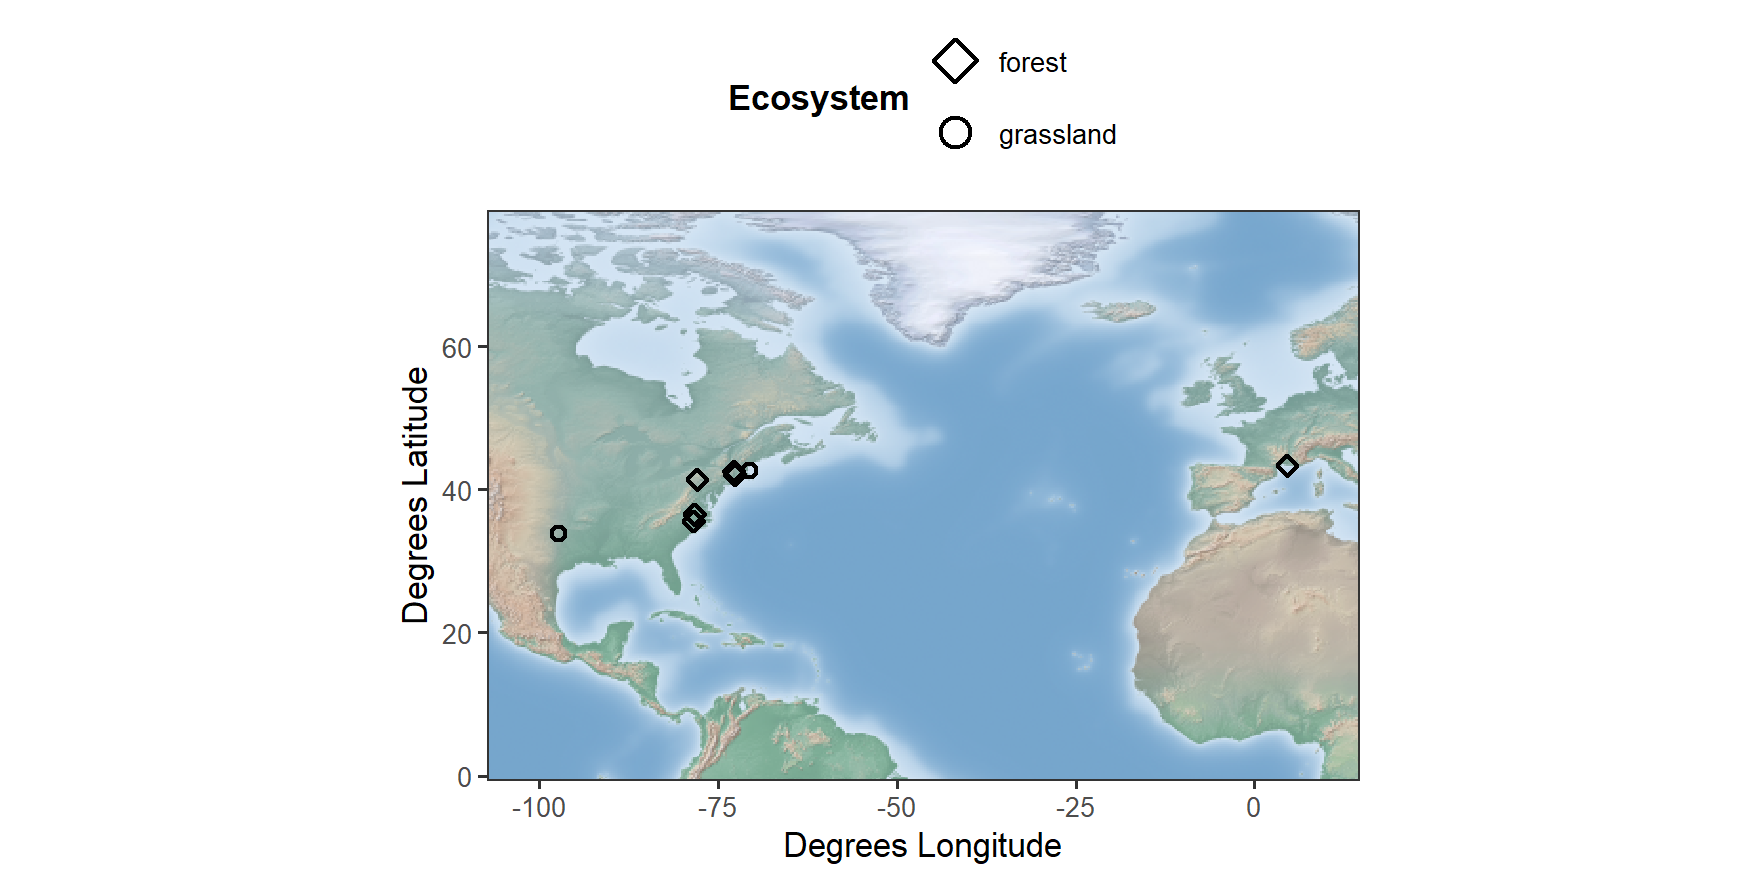
\includegraphics{../../Analyses/maps/soilms_experiments_map.png}
 \caption{\textbf{Map of locations of experiments included in this meta-analysis.Add phenophases to this- perhaps fill shapes by coloirs associated with phenophase}} 
 \label{fig:map}
 \end{figure}
 

\begin{figure}[h]
\centering
 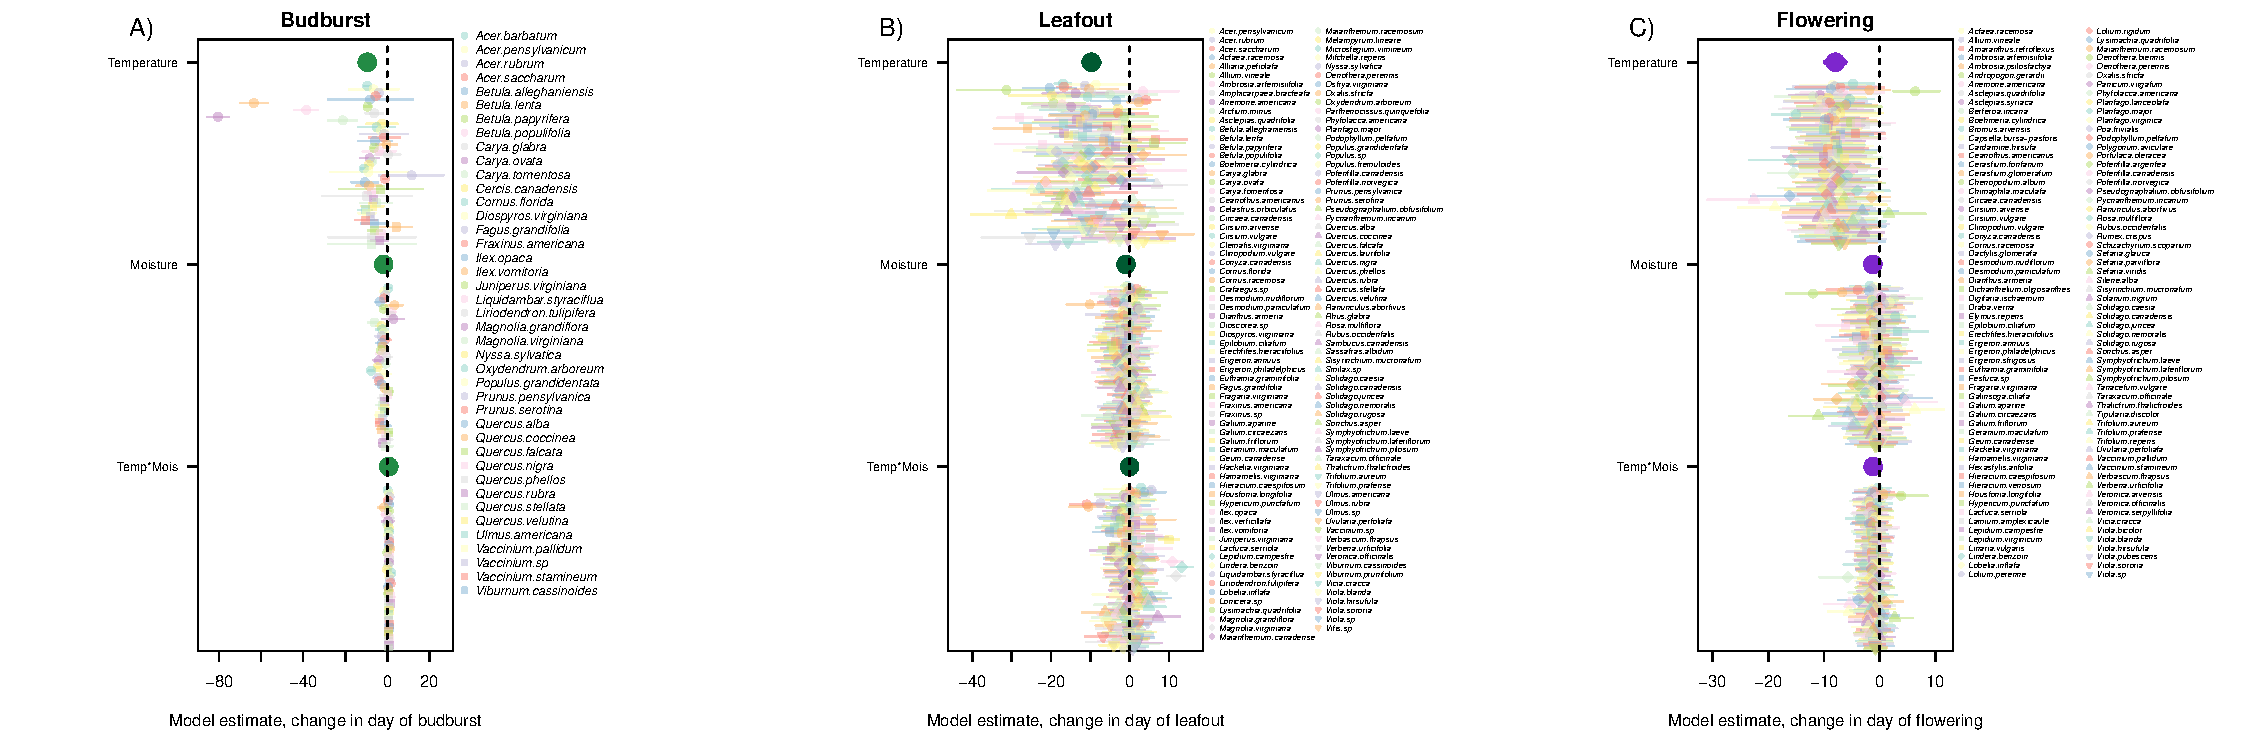
\includegraphics{../../Analyses/soilmoisture/figures/m5_bbdlofl.pdf}
 \caption{\textbf{Model coefficients from budburst, leafout, and flowering models (with centered predictors).}} 
 \label{fig:bblofl}
 \end{figure}
 

 \begin{figure}[h]
\centering
 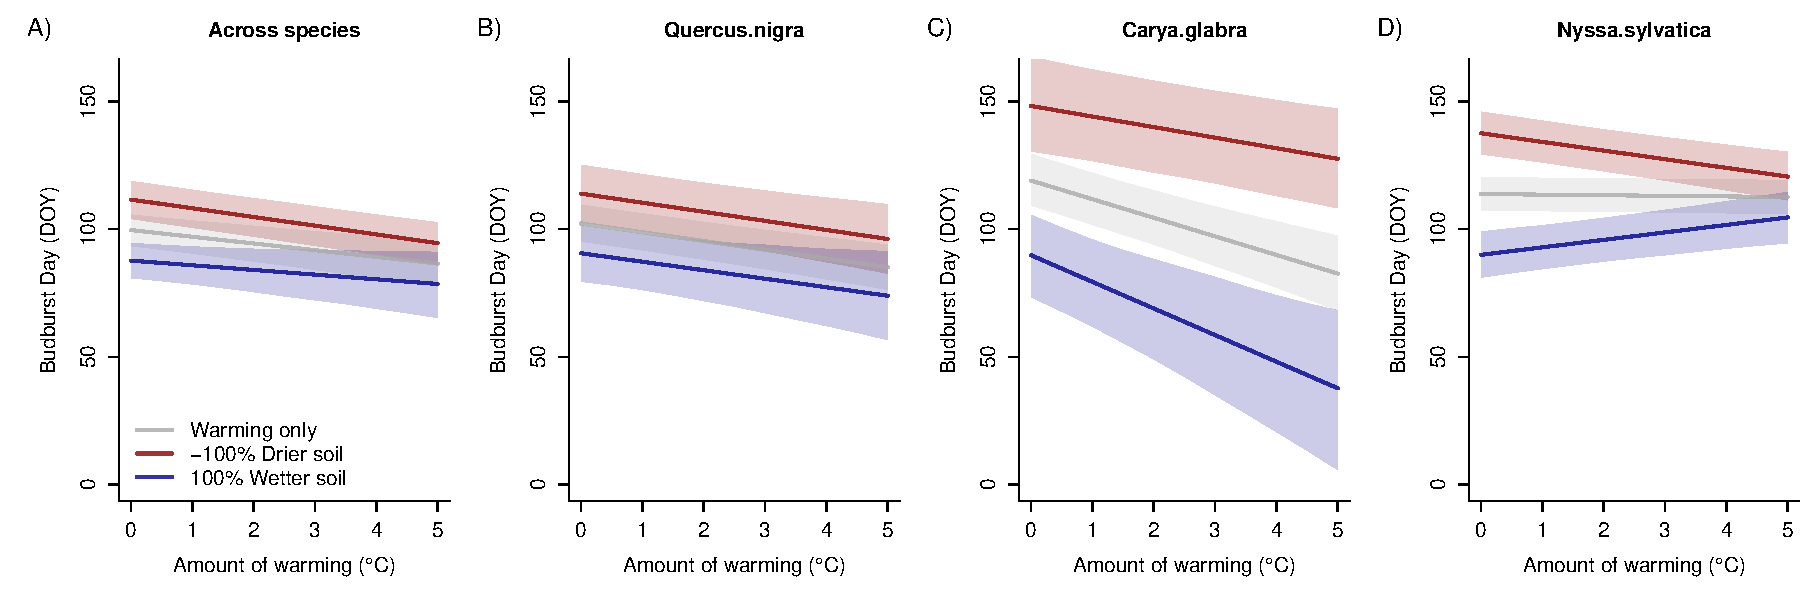
\includegraphics{../../Analyses/soilmoisture/figures/tempforecast_bb_0_5_135_28_105_4_degwarm.pdf}
 
 \caption{\textbf{Patterns of forecasted changes in budburst date with warming and shifts in soil moisture vary across species}. Across all species, our model estimated negative effects (i.e., earlier) of both temperature and soil moisture on budburst and a weak interaction between the two effects (A, and example species  \textit{Quercus nigra} in B); however, the magnitude of these effects, as well as the sign and magnitude of the estimated interaction between soil moisture and temperature, differed across species, resulting in divergent patterns with forecasted climate change.  Budburst may occur much earlier in wetter vs drier soils with warming for species that have a synergistic interaction between soil moisture and temperature, such as \textit{Carya glabra} (C). Whereas, other species with a antagonistic interaction, such as \textit{Nyssa sylvatica}(D), may experience delayed budburst in wet soils but advance in dry soils.}
 \label{fig:bbsp}
 \end{figure}

%%%%%%%%%%%%%%%%%%%%%%%%%%%%%%%%%%%%%%%%
\end{document}
%%%%%%%%%%%%%%%%%%%%%%%%%%%%%%%%%%%%%%%%


% Notes on some papers by Lizzie on 22 July 2022 -- on 24 July 2022 I deleted notes I already included above. 

\citep{howell202} "Altered precipitation treatments were only applied in early years of the study and neither precipitation treatments nor the treatments’ legacies significantly affected B. tectorum phenology." But warming did  advance flowering and shorten the vegetative season. % https://www.frontiersin.org/articles/10.3389/fpls.2020.570001/full

\citep{wang2022} "decreases in Pfreq during the past three decades positively contributed to the advance in LOD [leafout date] ... Notably, almost one-third of significant correlations (Pfreq versus LOD) for in situ and satellite data were negative (Fig. 2j-l), meaning that, for example, a decreased Pfreq comes with a delayed LOD"

\citep{tao2020} generally find same as us (they say negative relationship, but I finally tracked down what they mean -- "every 1\% m3/m3 increase in soil moisture led to a green-up date that was 3 to 6 days earlier"

\citep{Vitass2021} Did not get differences in soil moisture in their treatments

\citep{Crimmins:2010lv} "the decrease in autumn precipitation observed over the study period appears to explain the delay in onset observed for many of the species across the elevation gradient."

\citep{tao2019} "However, effects of precipitation and soil moisture on BBD varied among [herbaceous] species [in Inner Mongolia grassland]." ... "correlations between BBD and SM were negative, suggesting that greater soil moisture
would result in an earlier BBD." and it seems like mostly they did not find correlations otherwise; also their data are a gridded product

\cite{cabon2020} Good paper to cite for temperature and moisture being co-limiting .. hmm but they actually say "We found that temperature alone explains the onset of tracheid production" [and this is a modeling paper]

\cite{liu2022} If we need another example of complicated results from an experiment. 

\cite{sherry2007} " double precipitation treatment did not significantly affect flowering and fruiting phenology"

\cite{craine2012} most species flowering during warm wet times, but also discusses sort of divergence -- early versus late flowering species

\cite{wolkovich2012} says that exotic species advance with precip; while natives delay at Fargo and discusses drought avoidance strategies at Konza (where results diverge but are less significant)

\cite{seyed2018} "Across the entire study area, slow phenological development was associated with high MAT and moisture deficit (Fig. 4-a)."
